\section{Regulus}
\label{sec:regulus}

\subsection{Separation of Concerns}
The Regulus work has two main concerns. One is data and meta-data representations, manipulations and analysis. The second is a set of visualizations. Our design approach and implementation decisions for our analysis framework are described in \autoref{sec:app}, for the following, it is important to note that the framework consists of various types of visualizations, which the user can instantiate and connect to form an ever evolving set of well crafted coordinated multiple views. Multiple view instances of the same type (e.g. a tree view) can be used at the same time and they can refer to the same or different data. As such, the figures in the following usually depict a collage of screenshots. \todo[inline]{I wonder if we need this here. It depends on how many figures there will be}

Our aim is to identify interesting regions of input space as long as the output function behave approximately in a consistent way (quasi-monotonic). What constitute an interesting region depends on the domain or the questions an analyst is trying an answer. In the following we describe various examples of models, measures and analysis and how they can be used.

Previous works focused on creating consistent approximations of the output function over the whole domain. For each persistence level a new approximation is created. \autoref{fig:persistence-ui} shows an interface for selecting a persistence level. Issues: 1) a single value over the whole domain. 2) the main criterion is the apparent overall stability at certain persistence values 3) value selected only based on geometry. no consideration is given to other measures of the underlying partitions.

\subsection{Regulus Tree Perspective}
\todo[inline]{Need to find a better term for this}
A new perspective of a MS Complex hierarchy as a nested space partitions. 

At the base level (persistence = 0), the MS Complex consists of a set of space partitions. Each step of the simplification process cancels a pair of critical points causing several partition merges. Each merger consist of a pair of partitions where one partition subsume the other. In general, each cancellation leads to multiple mergers but a partition may participate in only one merger per cancellation. 

Instead of viewing the simplification process as mergers of critical points, we view them as mergers of partitions. The actual simplification process stays the same, it's only our perspectives that is changed. In contrast to the traditional perspective we do not view a merger as the assimilation of one partition into another, rather we treat the result of a merger as a new partition because the new partition describes a larger space partition with the combine set of points. The importance of this distinction arises when we fit a new model and apply various measures on the partitions as described in \ref{sec:measures}.

\subsection{Regulus Tree Layout}
\label{sec:tree}
The nested partitions constitute a binary tree, where each node represents a merger of two partitions (its children) at a given persistence value. 

There is a vast number of visualization technique to display trees.
Treemap only shows leaves with potentially titles of parent
icicle tree: no vertical or horizontal information

To the best of our knowledge the Regulus Tree visualization is novel. 

The Regulus Tree visualization consist of:
\begin{itemize}
    \item  We enumerate all the sample points along the horizontal axis based on the order of the leaves in the tree. The order within each base partition is not important

    \item We represent each leaf node by a rectangle that spans the collection of points in the corresponding partition

    \item A parent node represents the merger of its two children and since we arrange the children next to each other the parent rectangle span covers its two children

    \item  We layout the nodes vertically based on their persistence level such that the bottom of the rectangle is aligned with the persistence value when the two children are merged.

    \item  The height of a node encode the lifespan of the corresponding partition, that is, the rectangle extends up until its parent begins
\end{itemize}

\begin{figure}[htb]
    \begin{center}
     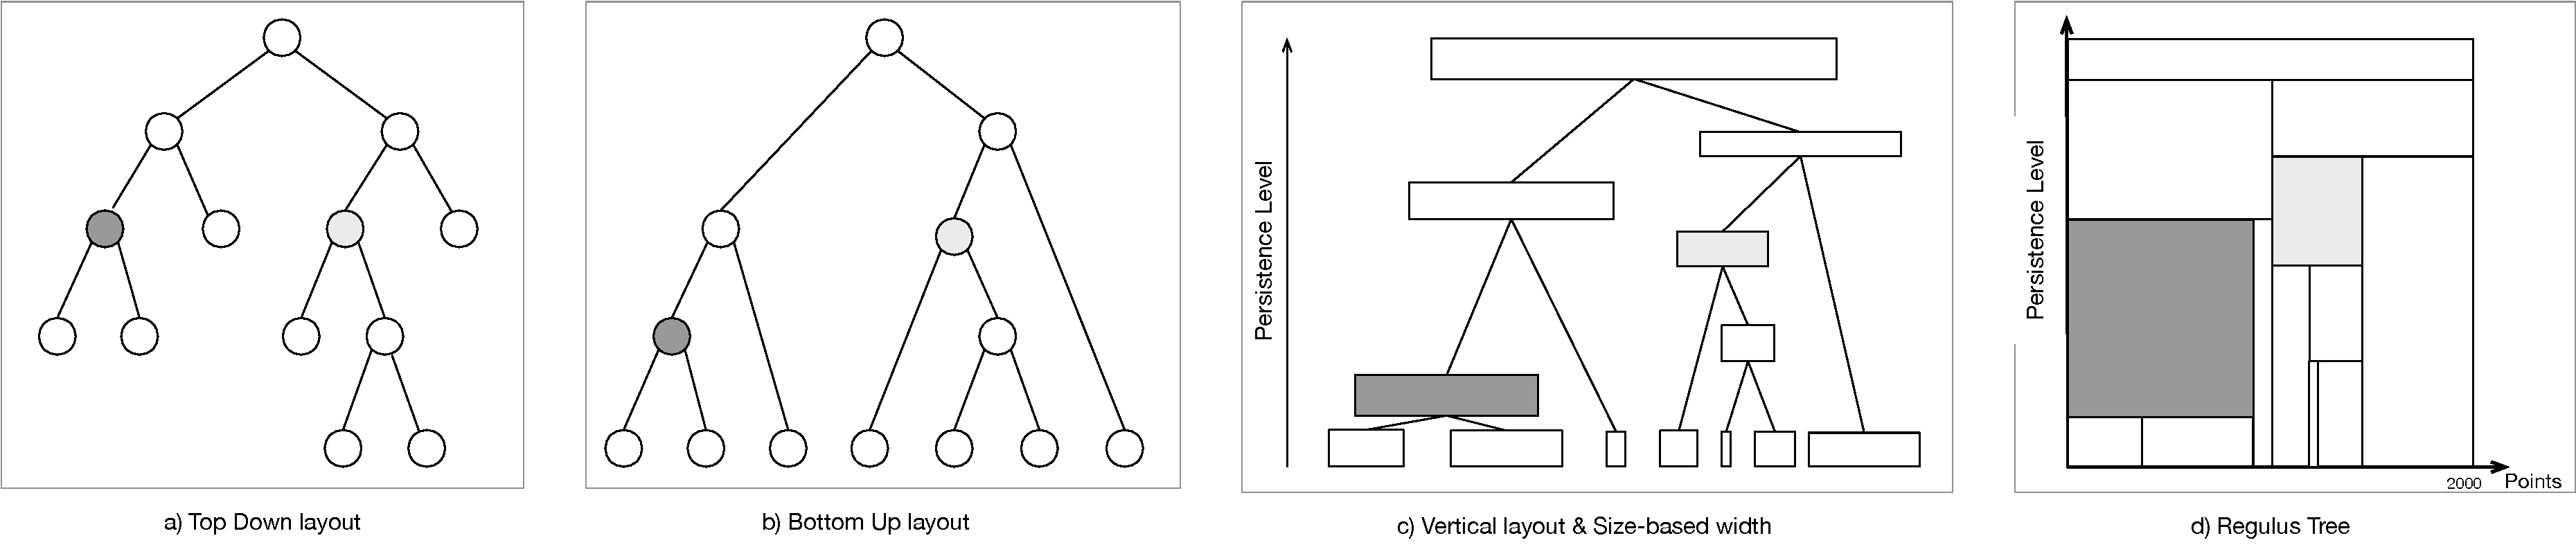
\includegraphics[width=\linewidth]{tree-diagram}
    \caption{The Regulus Tree layout: In a typical tree layout the nodes are positions based on their level as measured from the top (a) or bottom (b). Intermediate tree (c): Persistence is encoded by vertical position, size of partition is encoded by the width of a node.  Regulus tree (d): node height extends until parent to encode lifespan; horizontal layout based on enumeration of the points. Two of the nodes are shaded to illustrate the correspondence between the trees.}
    \label{fig:tree-diagram}
    \end{center}
\end{figure}

\begin{figure}[htb]
    \begin{center}
    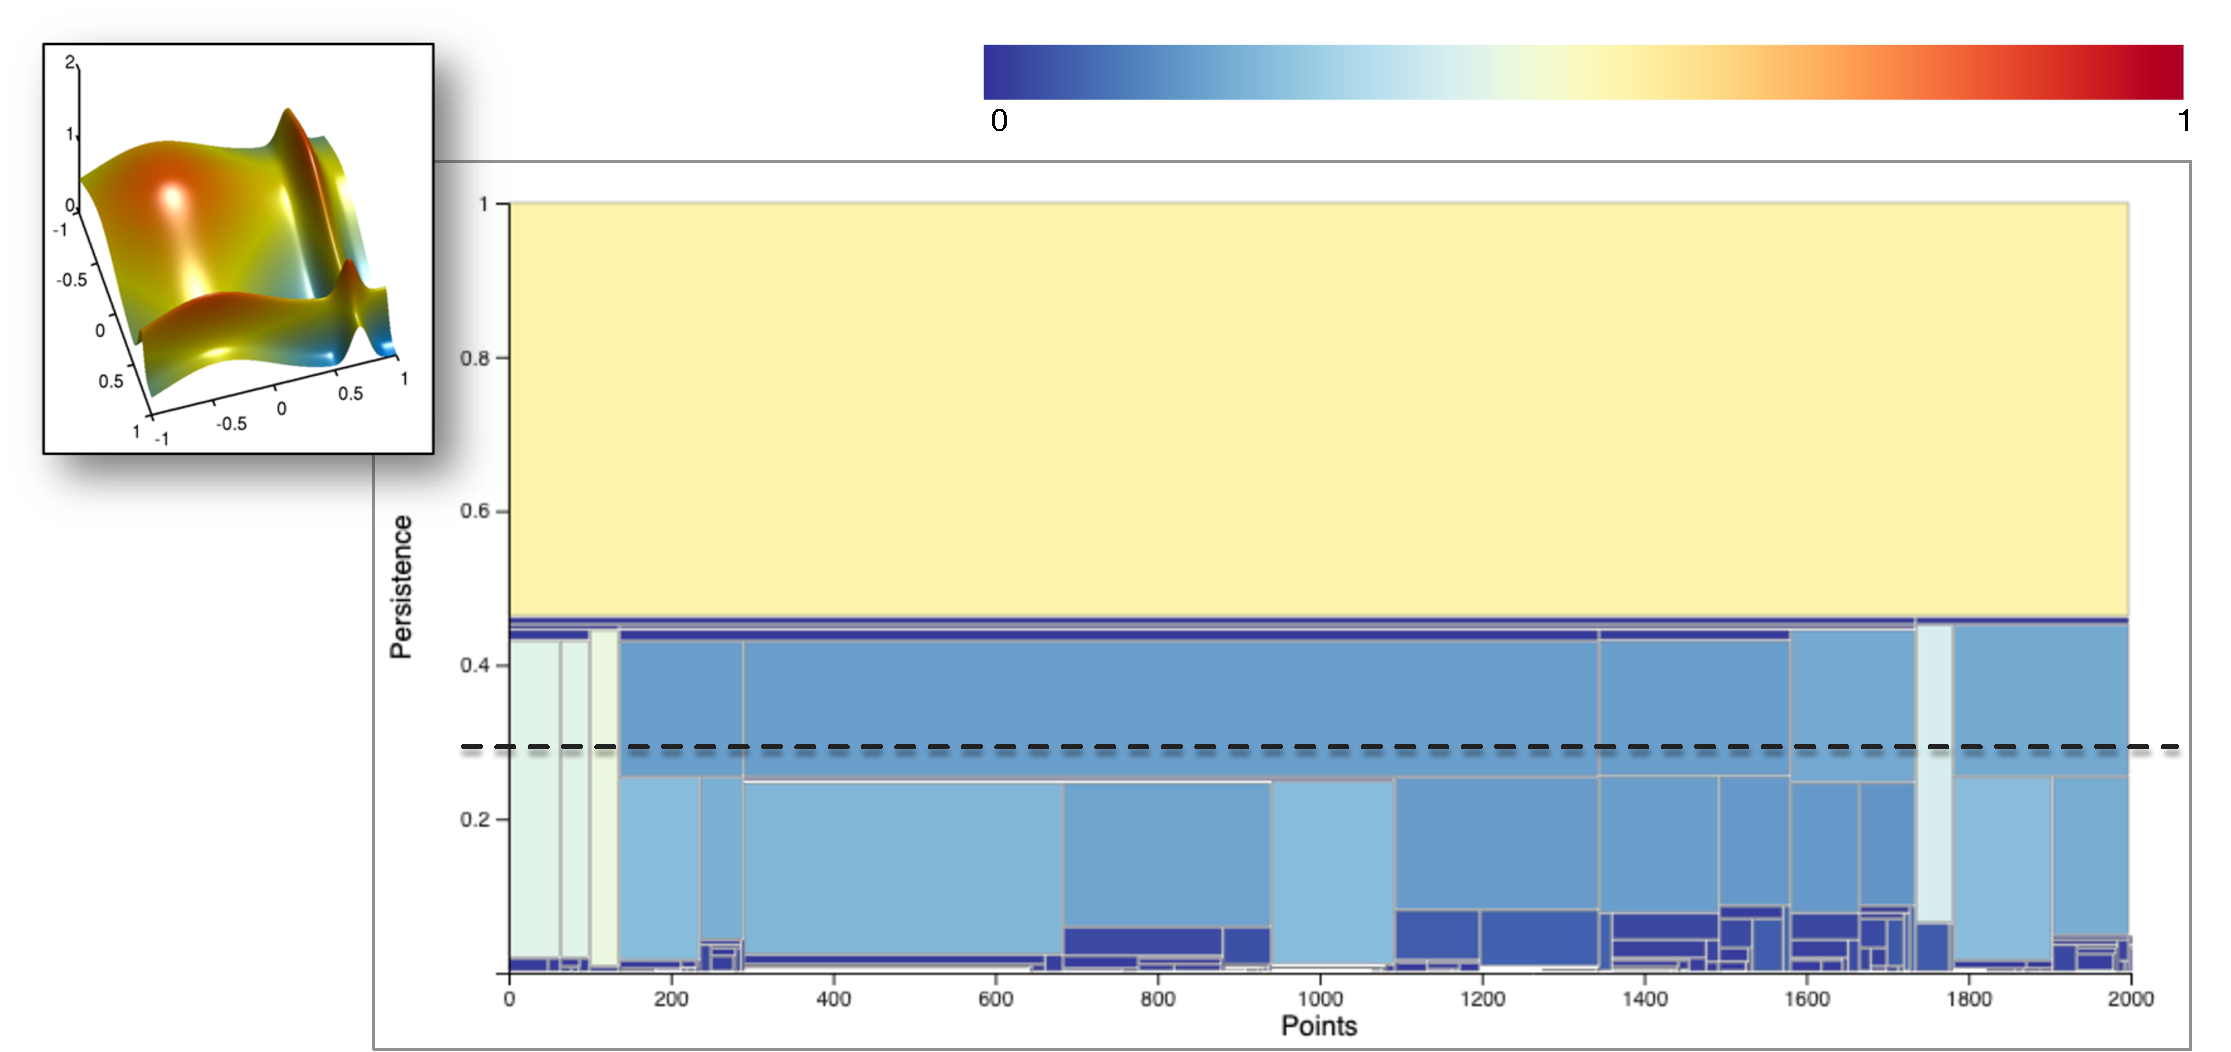
\includegraphics[width=\linewidth]{example}
    \caption{A 2D scalar function and a corresponding Regulus Tree. For illustration purpose, color encodes the lifespan of a partition using the blue-yellow-red colormap shown at the top. This is redundant, of course, as the same information is provided by the height of the node. For a persistence level of 0.3 the space decomposition consist of the nodes that intersect the dash line.}
    \label{fig:regulus-tree}
    \end{center}
\end{figure}
Arranging points sequentially such that each partition has 

Discuss the fact that extrema points are shared between partitions. We assign each extrema point to one base partition but each partition is aware of the extrema points

The Regulus Tree visualization provides a global view of all possible simplifications. For any given persistence value, the simplified space partitions, i.e. the collections of partitions at that level, are all the partitions in the Regulus Tree that intersect the horizontal line at that value as shown in ~\autoref{fig:regulus-tree}.


\subsection{Details View}
\label{sec:details}

Depicts projections of points in selected partitions. 

The inverse regression curves associated with the partition may be shown. Inverse regression curves are described in \autoref{sec:inverse-curves}.

Maybe describe the point filtering as was done in the JS version and have not been ported to the new version. 
\begin{itemize}
    \item One can filter by specifying a range in any input dimension, $x_i$
    \item range in the output dimension, $Y$, which will be repeated in all of the partitions
    \item selecting a range of points in a any of the panels. Note that in this case, the selection is based on actual points not range of values. As such, 
    \begin{itemize}
        \item the same points will be highlighted in a parent partition
        \item a subset (or all) of the points will be highlighted in a child partition
        \item no points will be highlighted in any other partition
    \end{itemize}
\end{itemize}
 

